% 1- Explicar detenidamente la principal motivacion del articulo. Dejar claro cual es el posible problema
% 2- Presentar las preguntas de investigacion pertinentes
% 3- Presentar algunos resultados preliminares
% 4- Presentar el trabajo llevado hasta ahora de investigacion y desarrollo
% 5- Dejar algunas preguntas abiertas y problemas encontrados hasta ahora
%
% $Id: slides.tex 4228 2006-06-21 21:55:12Z jjamor $
%
%
% Compilar a .pdf con LaTeX (pdflatex)
% Es necesario instalar Beamer (paquete latex-beamer en Debian)
%

%
% Grficos:
% Los grficos pueden suministrarse en PNG, JPG, TIF, PDF, MPS
% Los EPS deben convertirse a PDF (usar epstopdf)
%


\documentclass{beamer}
\usetheme{Warsaw}
\usebackgroundtemplate{
\includegraphics[width=\paperwidth]{format/libresoft-bg.png}}
\usepackage[english]{babel}
\usepackage[utf8]{inputenc}
\usepackage{graphics}
\usepackage{amssymb} % Simbolos matematicos
\usepackage{url}

%\definecolor{libresoftgreen}{RGB}{162,190,43}
%\definecolor{libresoftblue}{RGB}{0,98,143}

%\setbeamercolor{titlelike}{bg=libresoftgreen}

%% Metadatos del PDF.
\hypersetup{
  pdftitle={Libresoft},
  pdfauthor={Daniel Izquierdo Cort\'azar},
  pdfcreator={GSyC/Libresoft},
  pdfproducer=PDFLaTeX,
  pdfsubject={SQO-OSS and Alitheia Core},
}
%%



\AtBeginSection[]
{
  \begin{frame}<presentation>
    \frametitle{Index}
    \tableofcontents[current]
  \end{frame}
}




\begin{document}



\title{SQO-OSS and Alitheia Core
}
\subtitle{ Master on Free Software
}
\institute{jfelipe@libresoft.es\\
GSyC/Libresoft, Universidad Rey Juan Carlos}
\author{Felipe Ortega, Pedro Coca, Daniel Izquierdo Cort\'azar}
\date{Fuenlabrada, Madrid\\ 2nd, December 2010}

\frame{
\maketitle
\begin{center}

\includegraphics[width=4cm]{format/gsyc-urjc.pdf} 
\end{center}
}


% Si el titulo o el autor se quieren acortar para los pies de pgina
% se pueden redefinir aqu:
%\title{Titulo corto}
%\author{Autores abreviado}


%% LICENCIA DE REDISTRIBUCION DE LAS TRANSPAS
\frame{
~
\vspace{4cm}

\begin{flushright}
{\tiny
(cc) 2010 Felipe Ortega. \\
Some rights reserved. This document is distributed under the Creative \\
            Commons Attribution-ShareAlike 3.0 licence, available in \\
            http://creativecommons.org/licenses/by-sa/3.0/

%  Este documento (o uno muy similar) está disponible en \\
%  \url{http://gsyc.escet.urjc.es/~jjamor/}
}
\end{flushright}
}
%%

\frame{
\frametitle{Table of contents}
\tableofcontents
}


\section{Introduction}


\begin{frame}
\frametitle{Motivation}
\begin{center}
\begin{itemize}
\item Quality checking system for FLOSS projects.
\item Test quality of their code and relate this information with other data sources.
  \begin{itemize}
   \item Issue tracker
   \item Mailing list archives
   \item etc.
  \end{itemize}

\item Produces management-level information to assess various aspects of a software project, 
such as developer productivity.
\item Also useful for developers to check (and improve) quality of their code.
\item \texttt{http://www.sqo-oss.org}

\end{itemize}
\end{center}
\end{frame}



\begin{frame}
\frametitle{Alitheia}
\begin{center}
\begin{itemize}
\item Alitheia is the name of a platform, developed by the SQO-OSS project, for the automated 
objective evaluation of the quality of Open Source projects.
\item Analize ``hard'' and ``soft'' artifacts.
\begin{itemize}
 \item SCM is ``hard'' artifact (machine readable format, not aimed to humans).
 \item Mailing lists, issue trackes and other human communication tools are ``soft''.
\end{itemize}
\item \textit{Alitheia}: In Greek, the term stands for ``neat and businesslike truth''.

\end{itemize}
\end{center}
\end{frame}

\begin{frame}
\frametitle{Alitheia's goals}
\begin{center}
\begin{itemize}
\item Extensible platform.
\item Integrated representation of software engineering data.
\item First to automate and parallelize the execution of custom experiments.
\item No need to deal with low-level tasks such as pre-formatting data or updating 
their datasets when new data from projects become available

\end{itemize}
\end{center}
\end{frame}

\section{Design}

\begin{frame}
\frametitle{The system interface}
\begin{center}
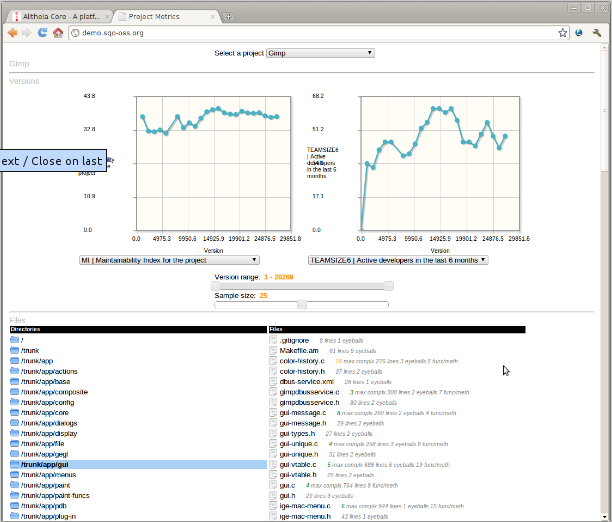
\includegraphics[width=0.8\textwidth]{figs/alitheia-snapshot.png}
\end{center}
\end{frame}

\begin{frame}
\frametitle{Alitheia design}
\begin{center}
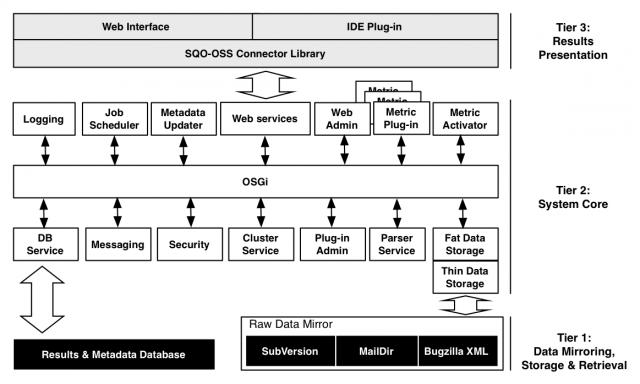
\includegraphics[width=0.9\textwidth]{figs/alitheia-design.png}
\end{center}
\end{frame}

\begin{frame}
\frametitle{Multilevel quality model}
\begin{center}
\begin{itemize}
\item Analyzability.
\item Changeability.
\item Stability.
\item Testability.
\item Maturity.
\item Effectiveness.
\item Security.
\item Mailing list.
\item Documentation.
\item Developer base.


\end{itemize}
\end{center}
\end{frame}

\begin{frame}
\frametitle{Evaluation}
\begin{center}
\begin{itemize}
\item Four categories:
\begin{itemize}
 \item Excellent (E)
 \item Good (G)
 \item Fair (F)
 \item Poor (P)
\end{itemize}
\item Where $E > G > F > P$
\end{itemize}
\end{center}
\end{frame}

\begin{frame}
\frametitle{Alitheia evaluation example}
\begin{center}
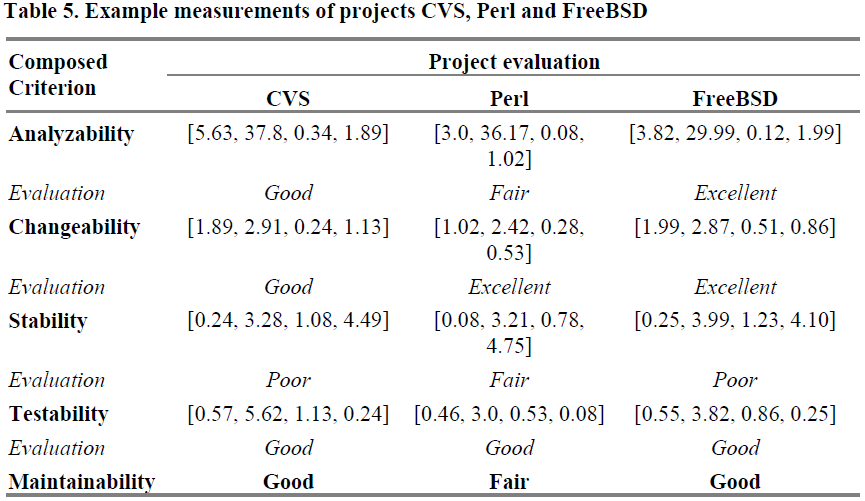
\includegraphics[width=0.9\textwidth]{figs/alitheia-eval-example.png}
\end{center}
\end{frame}

\begin{frame}
\frametitle{Alitheia metrics plug-ins lists}
\begin{center}
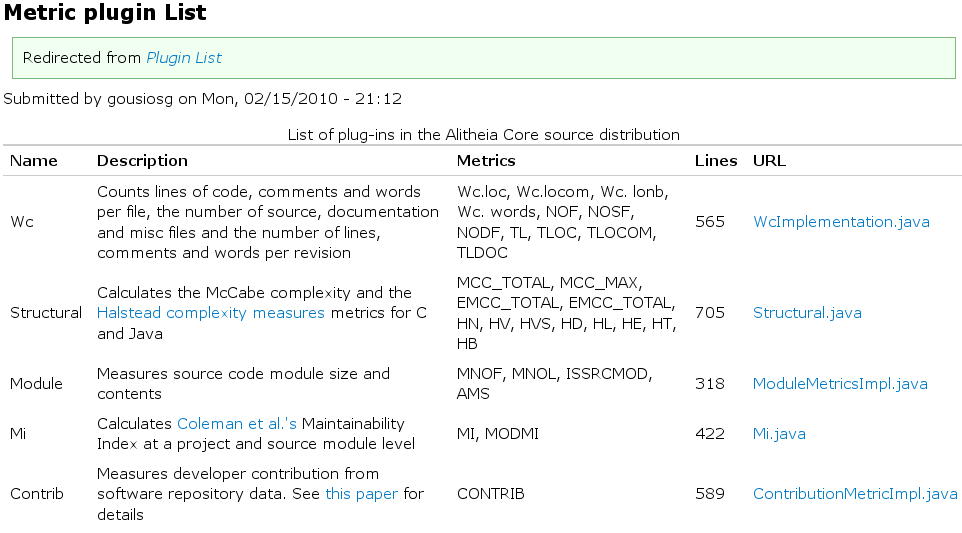
\includegraphics[width=0.9\textwidth]{figs/alitheia-metric-plugin-list.png}
\end{center}
\end{frame}

\section{Conclusions}

\begin{frame}
\frametitle{Conclusions}
\begin{center}
\begin{itemize}
\item Offers extensible platform to customize quality metrics.
\item Moved from a EU funded project to independently developed platform.
\item Lack of widespread support
\item Number of available plug-ins and documentation must be improved significantly.

\end{itemize}
\end{center}
\end{frame}


%**********************


\begin{frame}
\frametitle{Questions?}
\begin{center}
%Thanks for your attendance!\\
Questions?\\
%--\\
%\begin{small}
%Daniel Izquierdo Cortzar\\
%dizquierdo@gsyc.es\\
%GSyC/LibreSoft - Universidad Rey Juan Carlos\\
%\end{small}
\end{center}
\end{frame}




\end{document}
